\documentclass[border=3pt]{standalone}
\usepackage{circuitikz}
\usetikzlibrary{positioning}
\ctikzset{logic ports=ieee, logic ports/scale=0.9}
\begin{document}
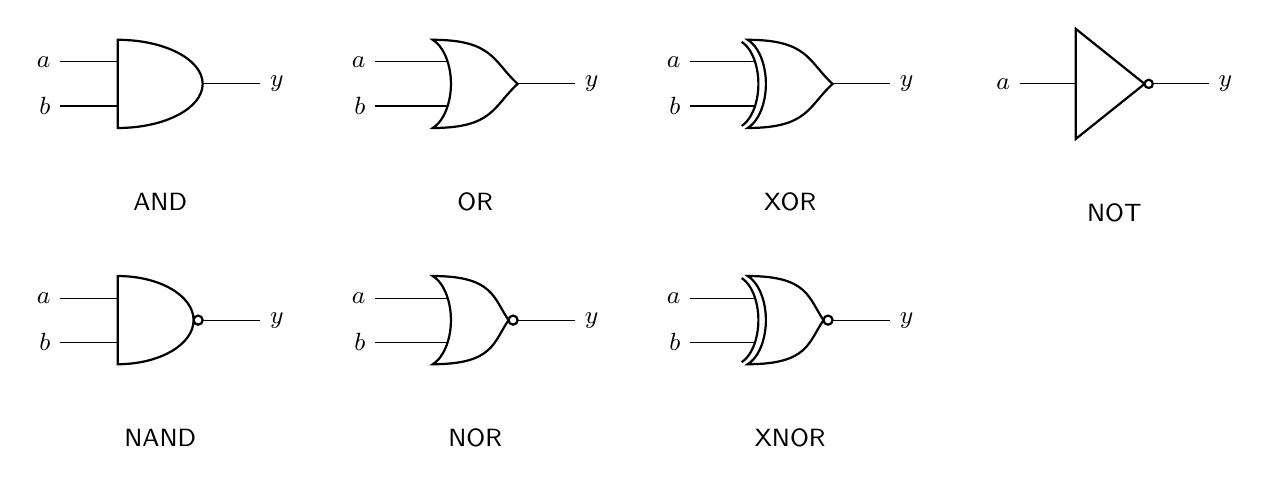
\begin{tikzpicture}[font=\sffamily\small]
  % AND
  \node[and port] (g1) at (0,0) {};
  \draw (g1.in 1) -- ++(-0.5,0) node[left]{$a$};
  \draw (g1.in 2) -- ++(-0.5,0) node[left]{$b$};
  \draw (g1.out) -- ++(0.5,0) node[right]{$y$};
  \node[below=7mm of g1]{AND};
  % OR
  \node[or port] (g2) at (4,0) {};
  \draw (g2.in 1) -- ++(-0.5,0) node[left]{$a$};
  \draw (g2.in 2) -- ++(-0.5,0) node[left]{$b$};
  \draw (g2.out) -- ++(0.5,0) node[right]{$y$};
  \node[below=7mm of g2]{OR};
  % XOR
  \node[xor port] (g3) at (8,0) {};
  \draw (g3.in 1) -- ++(-0.5,0) node[left]{$a$};
  \draw (g3.in 2) -- ++(-0.5,0) node[left]{$b$};
  \draw (g3.out) -- ++(0.5,0) node[right]{$y$};
  \node[below=7mm of g3]{XOR};
  % NOT
  \node[not port] (g4) at (11.5,0) {};
  \draw (g4.in) -- ++(-0.5,0) node[left]{$a$};
  \draw (g4.out) -- ++(0.5,0) node[right]{$y$};
  \node[below=7mm of g4]{NOT};
  % NAND
  \node[nand port] (g5) at (0,-3) {};
  \draw (g5.in 1) -- ++(-0.5,0) node[left]{$a$};
  \draw (g5.in 2) -- ++(-0.5,0) node[left]{$b$};
  \draw (g5.out) -- ++(0.5,0) node[right]{$y$};
  \node[below=7mm of g5]{NAND};
  % NOR
  \node[nor port] (g6) at (4,-3) {};
  \draw (g6.in 1) -- ++(-0.5,0) node[left]{$a$};
  \draw (g6.in 2) -- ++(-0.5,0) node[left]{$b$};
  \draw (g6.out) -- ++(0.5,0) node[right]{$y$};
  \node[below=7mm of g6]{NOR};
  % XNOR
  \node[xnor port] (g7) at (8,-3) {};
  \draw (g7.in 1) -- ++(-0.5,0) node[left]{$a$};
  \draw (g7.in 2) -- ++(-0.5,0) node[left]{$b$};
  \draw (g7.out) -- ++(0.5,0) node[right]{$y$};
  \node[below=7mm of g7]{XNOR};
\end{tikzpicture}
\end{document}
